\documentclass[12pt]{article}
\usepackage[utf8]{inputenc}
\usepackage{hyperref}
\usepackage{listings}
\usepackage{xcolor}
\usepackage{geometry}
\usepackage{graphicx} % For including graphics
\usepackage{minted} % For advanced code listings
\usepackage{listings-solidity}  % Include Solidity highlighting
\usepackage{amsmath, amssymb, amsfonts} % For mathematical equations


% Define a custom minted style (optional)
\usemintedstyle{colorful} % You can choose from various styles like 'monokai', 'tango', 'colorful', etc.

% Custom color setup
\definecolor{bashtextcolor}{RGB}{0, 0, 0} % Define black color

% Define a new command for inline code using minted
\newcommand{\codeinline}[1]{\mintinline{text}{#1}}

\geometry{a4paper, margin=1in}

\title{Smart Contracts Exercise 07: \\ Out of Gas}
\author{}
\date{}

% Define a new command for inline code with a dark background
\newcommand{\codeblack}[1]{%
  \texttt{\colorbox{black!7}{\textcolor{black}{#1}}}%
}

% Define a new command for inline code with a dark background
\newcommand{\codegrey}[1]{%
  \texttt{\colorbox{black!4}{\textcolor{black}{#1}}}%
}

% Define custom colors (optional)
\definecolor{myURLColor}{RGB}{0, 102, 204} % Example: A shade of blue

\hypersetup{
    colorlinks=true,        % Enable colored links
    linkcolor=blue,         % Color for internal links (e.g., \ref, \cite)
    citecolor=blue,         % Color for citations
    filecolor=magenta,      % Color for file links
    urlcolor=myURLColor     % Color for external URLs
}

% Define a style for code listings
\lstdefinestyle{mystyle}{
    backgroundcolor=\color{lightgray!20},   
    commentstyle=\color{green!50!black},
    keywordstyle=\color{blue},
    numberstyle=\tiny\color{gray},
    stringstyle=\color{red},
    basicstyle=\ttfamily\footnotesize,
    breakatwhitespace=false,         
    breaklines=true,                 
    captionpos=b,                    
    keepspaces=true,                 
    numbers=left,                    
    numbersep=5pt,                  
    showspaces=false,                
    showstringspaces=false,
    showtabs=false,                  
    tabsize=2
}

\lstset{style=mystyle}
% Adding package for header and footer
\usepackage{fancyhdr}
\pagestyle{fancy}

% Define header and footer
\fancyhf{} % Clear current settings
\fancyhead[L]{Smart Contracts Exercise 07} % Left header
\fancyhead[R]{\thepage} % Right header with page number

\renewcommand{\headrulewidth}{0.4pt} % Line below header
% \renewcommand{\footrulewidth}{0.4pt} % Line above footer

\begin{document}

\maketitle
\section{Introduction}

Denial of service attacks in smart contracts aim to render a contract
temporarily or permanently unusable by manipulating its execution flow or
exploiting resource limitations. Unlike traditional web applications where DoS
attacks typically involve overwhelming a system with traffic, blockchain DoS
attacks might be more sophisticated and can have permanent consequences. In
this exercise, you will learn about several types of DoS attacks on blockchain
and try to implement them in practical exercises. You will also become familiar
with the concept of decentralized autonomous organization.

\subsection*{Project Setup}

You have two options for working with this exercise: using a Docker container or
local installation. Choose the one that best fits your preferences.

\subsection{Using Docker with VS Code}

This option uses Docker to create a development environment with all the
necessary tools and dependencies preinstalled.

\subsubsection*{Prerequisites}

\begin{itemize}
    \item \textbf{\href{https://www.docker.com/products/docker-desktop}{Docker}} - A platform for developing, shipping, and running applications in containers.
    \item \textbf{\href{https://code.visualstudio.com/}{Visual Studio Code}} - A lightweight but powerful source code editor.
    \item \textbf{\href{https://marketplace.visualstudio.com/items?itemName=ms-vscode-remote.remote-containers}{Dev Containers}} - An extension to VS Code that lets you use a Docker container as a full-featured development environment.
\end{itemize}

\subsubsection*{Setting Up the Project:}

\begin{enumerate}
    \item Visit the following
          \href{https://gitlab.fel.cvut.cz/radovluk/smart-contracts-exercises/-/tree/main/07-Out-of-Gas/task/task-code}{GitLab
              repository} and clone it to your local machine.
    \item Open the repository folder in VS Code.
    \item When prompted, click ``Reopen in Container'' or use the command palette (F1)
          and run \codegrey{Dev Containers: Reopen in Container}.
\end{enumerate}

\subsection{Local Setup}

If you prefer working directly on your machine without Docker, you can set up
the development environment locally.

\subsubsection*{Prerequisites}
\begin{itemize}
    \item \textbf{Node.js}: \url{https://nodejs.org/en/} - An open-source, cross-platform, back-end JavaScript runtime environment that runs on the V8 engine and executes JavaScript code outside a web browser.
    \item \textbf{NPM}: Node Package Manager, which comes bundled with Node.js.
\end{itemize}

\noindent
Open your terminal and run the following commands to verify the installations:

\begin{minted}[bgcolor=gray!5, fontsize=\footnotesize]{bash}
$ node -v
$ npm -v
\end{minted}

Both commands should return the installed version numbers of Node.js and NPM
respectively. Node.js provides the runtime environment required to execute
JavaScript-based tools like Hardhat, while NPM is used to manage the packages
and dependencies needed for development.

\subsubsection*{Setting Up the Project}

\begin{enumerate}
    \item Visit the following
          \href{https://gitlab.fel.cvut.cz/radovluk/smart-contracts-exercises/-/tree/main/07-Out-of-Gas/task/task-code}{GitLab
              repository} and clone it to your local machine.
    \item Open a terminal and navigate to the project directory.
    \item Install the project dependencies by running \codegrey{npm install}.
\end{enumerate}

\section{Denial of Service Attacks}

Denial of Service (DoS) attacks in Ethereum smart contracts occur when a
malicious actor prevents legitimate users from using a contract's
functionality. There are several types of DoS attacks that can affect smart
contracts.

\subsection{DoS with Block Gas Limit}

Ethereum blocks have a maximum gas limit. If a function requires more gas than
this limit to execute, it becomes impossible to call that function. This commonly happens
with functions that loop through unbounded arrays, make multiple external
calls, or perform complex computations. Read more about gas:
\href{https://ethereum.org/gas/}{https://ethereum.org/gas/}.

The following code shows a contract that iterates through an unbounded array to
check if someone is a member of the organization. With each additional member
in the organization, the join function requires more and more gas to execute,
making it increasingly expensive to run. Eventually, when the member count
becomes too high, the join() function will become impossible to call due
to exceeding the block gas limit. You can try this yourself in the
\href{https://remix.ethereum.org/?#activate=solidity&url=https://github.com/radovluk/unbreakable-vault/contracts/DoS01.sol&lang=en&optimize=false&runs=200&evmVersion=null&version=soljson-v0.8.28+commit.7893614a.js}{prepared
    file in REMIX IDE}.

\noindent
\begin{minipage}{\textwidth}
    \begin{lstlisting}[language=Solidity, caption=DoS with Block Gas Limit Example]
contract Organisation {
    mapping(uint => address) members;
    uint public membersCount;
    uint public gasNeeded;

    function isMember(address addr) public view returns (bool) {
        for(uint i = 0; i < membersCount; i++) {
            if(members[i] == addr) return true;
        }
        return false;
    }

    function join() public {
        uint gas = gasleft();
        if(!isMember(msg.sender)) {
            members[membersCount++] = msg.sender;
        }
        gasNeeded = gas - gasleft();
    }
}
\end{lstlisting}
\end{minipage}

\subsection{DoS with Unexpected Revert}

When a contract requires all operations in a batch to succeed, a single
rejected operation can block the entire process. See this
\href{https://remix.ethereum.org/?#activate=solidity&url=https://github.com/radovluk/unbreakable-vault/contracts/DoS02.sol&lang=en&optimize=false&runs=200&evmVersion=null&version=soljson-v0.8.28+commit.7893614a.js}{example
    in REMIX IDE}. In this case, the successful execution of the \codegrey{claimThrone()}
function depends on the transfer operation completing successfully. If a smart
contract becomes the current king and doesn't implement a receive function, it
will remain the king forever.

\noindent
\begin{minipage}{\textwidth}
    \begin{lstlisting}[language=Solidity, caption=DoS with Revert Example]
contract KingOfEther {
    address public king;
    uint public balance;

    function claimThrone() external payable {
        require(msg.value > balance, "Need to pay more to become the king");
        payable(king).transfer(balance);
        balance = msg.value;
        king = msg.sender;
    }
}

contract MaliciousKing {    
    function attack(KingOfEther kingOfEther) external payable {
        kingOfEther.claimThrone{value: msg.value}();
    }

    // No receive function - will cause DoS when transfer is attempted
}
\end{lstlisting}
\end{minipage}

\subsection{Owner Operations DoS}

If a contract relies on an owner for critical operations and the owner's
private key is lost or the owner becomes unresponsive, the contract can become
permanently unusable.

\noindent
\begin{minipage}{\textwidth}
    \begin{lstlisting}[language=Solidity, caption=Owner Operations DoS Example]
function withdrawFunds() public onlyOwner {
    // What if the owner loses their private key?
    payable(owner).transfer(address(this).balance);
}
\end{lstlisting}
\end{minipage}

\noindent
In this example, if the owner loses their private key or becomes unresponsive, the funds are permanently locked.

\subsection{DoS Mitigation Strategies}

\subsubsection*{Pull Over Push Payment Pattern}

Instead of pushing payments to users, let users pull their own funds. This
pattern shifts the responsibility of handling failed transactions to individual users
rather than affecting everyone.

\noindent
\begin{minipage}{\textwidth}
    \begin{lstlisting}[language=Solidity, caption=Pull Over Push Example]
mapping(address => uint256) public pendingWithdrawals;

// Allow users to claim their funds individually
function withdraw() public {
    uint amount = pendingWithdrawals[msg.sender];
    // Remember to set pending withdrawals to 0 before transfer
    pendingWithdrawals[msg.sender] = 0;
    payable(msg.sender).transfer(amount);
}
\end{lstlisting}
\end{minipage}

\subsubsection*{Avoid Unbounded Operations}

Avoid iterating through unbounded arrays or performing unbounded operations that
could exceed the block gas limit.

\noindent
\begin{minipage}{\textwidth}
    \begin{lstlisting}[language=Solidity, caption=Bounded Operations Example]
function processBatch(uint start, uint batchSize) public {
    // Process only a limited number of items per transaction
    uint end = start + batchSize;
    require(end <= array.length, "Invalid batch");
    
    for(uint i = start; i < end; i++) {
        // Process items in batches
        processItem(array[i]);
    }
}
\end{lstlisting}
\end{minipage}

\subsubsection*{External Calls Handling}

When making external calls, handle failures gracefully without causing the
entire function to revert.

\noindent
\begin{minipage}{\textwidth}
    \begin{lstlisting}[language=Solidity, caption=Safe External Call Example]
function processPayments() public {
    for(uint i = 0; i < recipients.length; i++) {
        // Note missing require statement - we continue even if one transfer fails
        (bool success, ) = recipients[i].call{value: amounts[i]}("");
        if(success) {
            emit PaymentSuccessful(recipients[i], amounts[i]);
        } else {
            emit PaymentFailed(recipients[i], amounts[i]);
            // Store failed payments for later retry
            failedPayments[recipients[i]] = amounts[i];
        }
    }
}
\end{lstlisting}
\end{minipage}

\section{Decentralized Autonomous Organizations (DAOs)}

DAOs are blockchain-based organizations governed by smart contracts and
controlled by their members rather than by a central authority. They rely on
on-chain voting mechanisms to make decisions and allocate resources. The
foundation of a DAO is a smart contract on the blockchain that precisely
establishes the rules by which the organization will be governed. Examples of
DAOs include charities (where members decide where to contribute funds),
collective ownership structures, and ventures and grants - where venture funds
pool investment capital and members vote on which ventures to support. Key
components of DAOs include:

\begin{enumerate}
    \item \textbf{Membership Management}: Rules for joining the DAO, often by holding governance tokens or paying membership fees.
    \item \textbf{Proposal Mechanism}: Allowing members to submit proposals for changes or funds allocation.
    \item \textbf{Voting System}: A system for members to vote on proposals.
    \item \textbf{Execution Mechanism}: Logic for implementing approved proposals.
\end{enumerate}

\noindent
One of the most infamous DAO organizations was the notorious \href{https://en.wikipedia.org/wiki/The_DAO}{The DAO}, which you learned about in Exercise 05 - Re-entrancy. You will see a simple example of a DAO in Task 2.

\begin{table}[H]
    \centering
    \footnotesize
    \begin{tabular}{|p{0.40\textwidth}|p{0.40\textwidth}|}
        \hline
        \multicolumn{1}{|c|}{\textbf{DAO}}                                                                                      & \multicolumn{1}{c|}{\textbf{Traditional Organization}}                                           \\
        \hline
        Usually flat, and fully democratized.                                                                                   & Usually hierarchical.                                                                            \\
        \hline
        Voting required by members for any changes to be implemented.                                                           & Depending on structure, changes can be demanded from a sole party, or voting may be offered.     \\
        \hline
        Votes tallied, and outcome implemented automatically without trusted intermediary.                                      & If voting allowed, votes are tallied internally, and outcome of voting must be handled manually. \\
        \hline
        Services offered are handled automatically in a decentralized manner (for example distribution of philanthropic funds). & Requires human handling, or centrally controlled automation, prone to manipulation.              \\
        \hline
        All activity is transparent and fully public.                                                                           & Activity is typically private, and limited to the public.                                        \\
        \hline
    \end{tabular}
    \caption{DAOs and Traditional Organizations (from: \href{https://ethereum.org/dao/}{Ethereum.org})}
    \label{tab:dao-comparison}
\end{table}

\medskip
\noindent
More about DAOs:
\begin{itemize}
    \item \textbf{Read:} \href{https://ethereum.org/dao/#what-are-daos}{What is a DAO?}
    \item \textbf{Video:} \href{https://www.youtube.com/watch?v=KHm0uUPqmVE}{What is a DAO in Crypto?}
    \item \textbf{TED Talk:} \href{https://www.youtube.com/watch?v=zTStDvUtQWc}{Could a DAO Build the Next Great City?}
\end{itemize}

\section{Task}

\subsection*{Task 1: NFT Auction Sabotage}

One of the most valuable students from the FEL NFT Students collection is now
for sale. It depicts an Electronics and Communication student who dozed off with a
calculator. The owner (seller) has decided not to sell this rare piece on an
ordinary marketplace but through an auction. The starting price is 0.5 ETH,
but it quickly rises to 2.8 ETH. You have 3 ETH available and want to acquire
this piece at all costs! Suddenly, a well-known speculator and reseller appears
and announces on the auction forum that they'll pay 50 ETH for the NFT student.
You realize that you no longer have any chance of winning the auction. But you
decide: if you can't have the NFT, no one will!

\begin{figure}[h!]
    \centering
    \begin{minipage}{0.3\textwidth}
        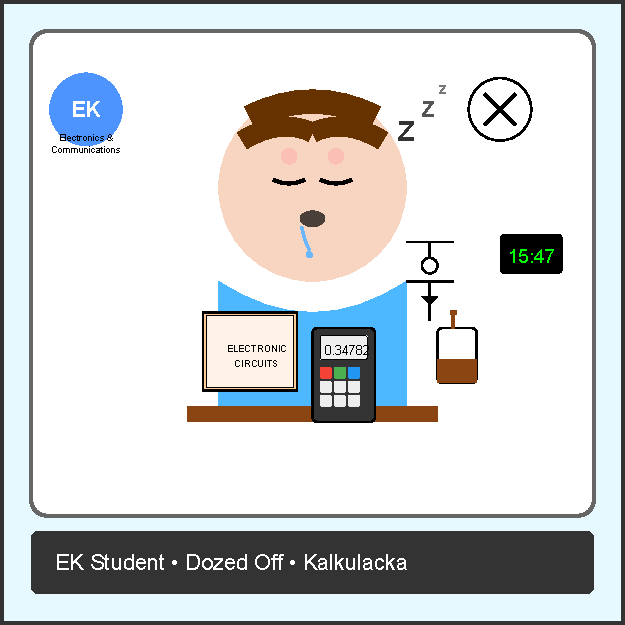
\includegraphics[width=\textwidth]{NFTs/ek-student-nft.pdf}
    \end{minipage}
\end{figure}

\medskip
\noindent
\textbf{Your Mission:}
\begin{itemize}
    \item Prevent the reseller from acquiring the NFT Student - your code will run before
          the reseller (bidder 3) places their 50 ETH bid
    \item Ensure that none of the other auction participants can acquire the NFT Student
          either
\end{itemize}

\noindent
Code your solution in the \texttt{test/NFTAuction.js} file. Use only the player account or contracts that you deploy using the player account. Verify your solution by running the following command:

\begin{minted}[bgcolor=gray!5, fontsize=\footnotesize]{bash}
$ npm run auction
\end{minted}

\noindent
Files that are relevant for this challenge:
\begin{itemize}
    \item test/\textbf{NFTAuction.js}: The test file where you should code your solution.
    \item contracts/\textbf{NFTAuction.sol}: The auction contract where the auction is
          taking place.
    \item contracts/\textbf{FELStudentNFT.sol}: The NFT collection contract.
\end{itemize}

\subsection*{Task 2: Save the DAO Funds From the Cats}

You decided to join a DAO with other people to collectively manage your
finances. The founder of the DAO contributed 10 ETH, and anyone who wants to
join the DAO must pay a membership fee of 1 ETH. Everything looks promising
until one member proposes to donate all the funds to a cat charity
organization. This proposal is very popular and all members (except you) vote
in favor of it. By coincidence, it's the same cat charity that you exploited in
Exercise 4, but this time it's sufficiently protected against reentrancy
attacks. You hate cats and don't want the funds to reach them under any
circumstances.

\medskip
\noindent
\textbf{Your Mission:}
\begin{itemize}
    \item Prevent the execution of the proposal to donate funds to the cat charity
    \item Ensure the treasury funds remain in the DAO
    \item You have 1.5 ETH available to achieve this goal
\end{itemize}

\noindent
Code your solution in the \texttt{test/DAO.js} file. Use only the player account, which is already a DAO member.  Verify your solution by running the following command:

\begin{minted}[bgcolor=gray!5, fontsize=\footnotesize]{bash}
$ npm run dao
\end{minted}

\noindent
Files that are relevant for this challenge:
\begin{itemize}
    \item test/\textbf{DAO.js}: The test file where you should code your solution.
    \item contracts/\textbf{DAO.sol}: The contract forming your Decentralized Autonomous
          Organization.
    \item contracts/\textbf{CatCharity.sol}: The cat charity contract. You do not need to
          pay any special attention to this contract.
\end{itemize}

\end{document}
